\chapter{Trabalhos Relacionados}

\section{Introdução}

Este capítulo apresenta os trabalhos relacionados à utilização de RNC para treinamento de imagens, com e sem variação de parâmetros; a trabalhos que aplicam especificamente a versão 8 do YOLO; aqueles que utilizaram VANT e os que criaram automação para sistemas de Realidade Virtual. O objetivo é encontrar o estado da arte de cada trabalho, destacando as principais contribuições.

No final do capítulo, os estudos são comparados para justificar o sistema abordado neste trabalho.

\section{Alteração de Parâmetros da RNC}
\subsection{Identificação e Medição de Defeitos em Produtos Automotivos Usando Visão Computacional}

A dissertação apresentada por \cite{gonzaga2023identificaccao} investigou a aplicabilidade e eficiência de um sistema de visão computacional para identificar defeitos visuais no controle de qualidade de peças automotivas reposição. O intuito do trabalho foi de avaliar a possibilidade de automatizar de modo confiável o processo de inspeção e precificação do reparo destas peças.

Para este trabalho, foi utilizado um dataset composto por imagens de vidros automotivos, fornecidos por uma empresa do ramo. Os defeitos analisados incluíram bolhas, delaminação, irisação, ostra e grau em vidros, além de manchas em peças como faróis, lanternas e retrovisores. Todos esses defeitos foram identificados nas fotos fornecidas. Assim como na presente dissertação, foi utilizado o software LabelImg para realizar a marcação da ocorrência de cada uma dessas anomalias no conjunto de fotos, como se vê na Figura \ref{fig:mancha}.

\begin{figure}[!h]
    \center
    \begin{minipage}{1\linewidth}
        \center
        \captionsetup{justification=centering,margin=0.5cm,font=small}
        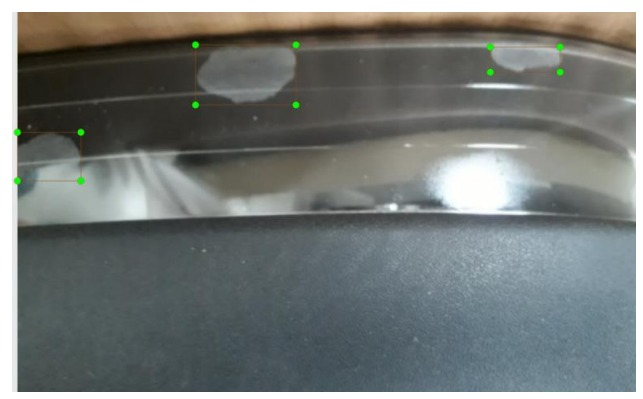
\includegraphics[width=0.7\linewidth]{img/cap3/mancha-marcacao.jpeg}
        \caption{Exemplo de marcação de foto utilizando labelImg, de um defeito em um vidro \cite{gonzaga2023identificaccao}}
        \label{fig:mancha}
    \end{minipage}
\end{figure}

Em sua fundamentação, foram entendidas as RNC como ferramentas eficazes para o processamento de imagens. Avaliou-se a rede ResNet \cite{he2016deep}, como uma possibilidade de arquitetura para processar as imagens, justamente por se mostrar uma ferramenta poderosa para a identificação de padrões. Para tanto, ela se vale de uma série de camadas residuais com conexões de salto, permitindo que os gradientes fluam mais facilmente através da rede durante o treinamento, mitigando o problema do desaparecimento do gradiente. Esse problema ocorre quando, em redes profundas, os gradientes se tornam extremamente pequenos ao retropropagar através das camadas, dificultando a atualização dos pesos nas camadas iniciais e, consequentemente, a aprendizagem adequada da rede. A ResNet supera essa dificuldade utilizando conexões que pulam uma ou mais camadas, somando a entrada diretamente à saída dessas camadas puladas, permitindo a construção de redes muito mais profundas sem a degradação do desempenho (Figura \ref{fig:salto}). Com isso, a ResNet consegue capturar e aprender padrões complexos presentes nas imagens, resultando em uma melhoria significativa na precisão das tarefas de classificação e reconhecimento de imagens.
	
\begin{figure}[!h]
    \center
    \begin{minipage}{1\linewidth}
        \center
        \captionsetup{justification=centering,margin=0.5cm,font=small}
        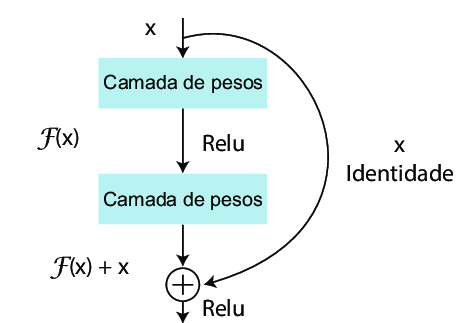
\includegraphics[width=0.7\linewidth]{img/cap3/salto.png}
        \caption{Bloco de aprendizado da ResNet \cite{he2016deep}}
        \label{fig:salto}
    \end{minipage}
\end{figure}

Contudo, a ResNet, devido à sua grande quantidade de camadas e processamento, acaba por ser morosa durante o treinamento. Além disso, sua utilização não é trivial e exige configurações específicas. Deste modo, o trabalho explora as vantagens da YOLO como alternativa. A YOLO é extremamente rápida, treinando em imagens completas com uma única passagem pelas imagens, o que reduz significativamente o tempo de processamento. Sua arquitetura simples e eficiente permite a detecção de múltiplos objetos em uma única passagem pela rede, tornando o treinamento mais direto e eficaz em termos de recursos computacionais. Além disso, a YOLO é altamente generalizável e menos propensa a erros de background, sendo uma solução mais prática e veloz para detecção de objetos.	

Para o treinamento, foram analisadas 3.397 imagens com defeitos específicos da rotina da empresa. Destas, 70\% foram utilizadas para treinamento e 30\% para validação. Todas as imagens foram anotadas manualmente. Em cada uma delas, pelo menos um dos defeitos estudados deveria constar nela para que a imagem fosse colocada para treinamento. Essa parte do processo garantiu que o modelo gerado fosse significativo.

Além disso, foram variados os tamanhos do valor do \textit{batch size} (entre 2 e 32) e testados três otimizadores diferentes: SGD, Adam e AdamW. A YOLOv5 oferece variações da arquitetura para diferentes propósitos. Neste trabalho, foram testadas 10 variações da arquitetura, juntamente com a alteração de parâmetros. Todos os outros hiperparâmetros foram mantidos na configuração padrão. Cada treinamento foi realizado em 300 épocas.

Na Tabela \ref{tab:resultado-mancha}, é apresentado o resultado do treinamento, com os respectivos valores, com a variação de parâmetro. Nota-se, disso, que o otimizador SGD, na variação YOLOv5x, com batch size de 8, alcançou a melhor precisão média, com mAP de 0,72921, mostrando com isso a melhor configuração. Com esse treinamento aplicado na identificação de imagens, resultou-se em 83,33\% de precisão na precificação correta dos produtos defeituosos, mostrando com isso que a automação foi bem sucedida em seu propósito.

\begin{table}[h!]
    \label{tab:resultado-mancha}
    \centering
    \begin{tabular}{|c|c|c|c|c|}
    \hline
    \multicolumn{5}{|c|}{\textbf{Otimização Adam}} \\ \hline
    \textbf{ARQUITETURA} & \textbf{Batch 2} & \textbf{Batch 4} & \textbf{Batch 8} & \textbf{Batch 16} \\ \hline
    YOLOv6n  & 0.27538 & 0.34865 & 0.38961 & 0.41800 \\ \hline
    YOLOv5n  & 0.34196 & 0.36812 & 0.34965 & 0.44277 \\ \hline
    YOLOv6s  & 0.29176 & 0.29275 & 0.34995 & 0.39963 \\ \hline
    YOLOv5s  & 0.22021 & 0.27696 & 0.30976 & 0.40907 \\ \hline
    YOLOv6m  & 0.22398 & 0.29198 & 0.33198 & 0.42154 \\ \hline
    YOLOv5m  & 0.26330 & 0.31970 & 0.38044 & 0.44705 \\ \hline
    YOLOv6l  & 0.22940 & 0.30710 & 0.34329 & 0.44475 \\ \hline
    YOLOv6n  & 0.30030 & 0.39497 & - & - \\ \hline
    YOLOv5x  & 0.32160 & 0.38688 & - & - \\ \hline
    
    \multicolumn{5}{|c|}{\textbf{Otimização AdamW}} \\ \hline
    \textbf{ARQUITETURA} & \textbf{Batch 2} & \textbf{Batch 4} & \textbf{Batch 8} & \textbf{Batch 16} \\ \hline
    YOLOv6n  & 0.42883 & 0.43552 & 0.49657 & - \\ \hline
    YOLOv5n  & 0.48022 & 0.48880 & 0.57565 & - \\ \hline
    YOLOv6s  & 0.44942 & 0.49605 & 0.58261 & - \\ \hline
    YOLOv5s  & 0.43433 & 0.52185 & 0.55821 & - \\ \hline
    YOLOv6m  & 0.51829 & 0.53139 & 0.60474 & - \\ \hline
    YOLOv5m  & 0.46789 & 0.50103 & 0.58947 & - \\ \hline
    YOLOv6l  & 0.46769 & 0.50310 & 0.58947 & - \\ \hline
    YOLOv6n  & - & - & - & - \\ \hline
    YOLOv5x  & - & - & - & - \\ \hline
    
    \multicolumn{5}{|c|}{\textbf{Otimização SGD}} \\ \hline
    \textbf{ARQUITETURA} & \textbf{Batch 2} & \textbf{Batch 4} & \textbf{Batch 8} & \textbf{Batch 16} \\ \hline
    YOLOv6n  & 0.57286 & 0.55400 & 0.65654 & - \\ \hline
    YOLOv5n  & 0.59021 & 0.60678 & 0.60235 & - \\ \hline
    YOLOv6s  & 0.60723 & 0.61912 & 0.61684 & - \\ \hline
    YOLOv5s  & 0.67145 & 0.70897 & 0.71185 & - \\ \hline
    YOLOv6m  & 0.60228 & 0.71413 & 0.71037 & - \\ \hline
    YOLOv5m  & 0.61179 & 0.71564 & 0.70514 & - \\ \hline
    YOLOv6l  & 0.62377 & 0.71564 & 0.70514 & - \\ \hline
    YOLOv6n  & 0.71112 & 0.71067 & - & - \\ \hline
    YOLOv5x  & 0.70527 & 0.71120 & - & - \\ \hline
    
    \end{tabular}
    \caption{Tabela comparativa de desempenho de modelos YOLO com diferentes otimizações e tamanhos de batch.}
    \end{table}
    

\section{Aplicação YOLOv8}
\subsection{Comparação de Modelos YOLOv5 e YOLOv8 para Detecção de Objetos em Áreas Rurais Usando Transferência de Aprendizado}

O artigo de \cite{diascomparaccao}, apresenta um estudo comparativo entre duas versões da YOLO, a YOLOv5 e YOLOv8. Nele, avalia-se o desempenho de ambos os modelos na detecção de objetos em cenários característicos de ambientes rurais, onde os desafios incluem a presença de objetos agrícolas, plantações, animais e estruturas. Além disso, é utilizada uma técnica de transferência de aprendizado com modelos pré-treinados para adaptar ambas arquiteturas ao contexto proposto.

Como embasamento teórico, buscou-se um estudo similar ao apresentado, em que foi realizada também uma comparação dos modelos YOLOv5 e YOLOv8 para detecção de veículos e placas em sistemas de transporte inteligentes, usando transferência de aprendizado com dados da plataforma Kaggle \cite{afonso2023vehicle}. Após uma avaliação abrangente, concluíram que o YOLOv8 superou ligeiramente o YOLOv5, além de ter um tempo de treinamento menor.

Já no trabalho citado de \cite{silva2018detecccao}, foi estudada a detecção e contagem de plantas usando inteligência artificial, aplicando modelos de visão computacional para detectar e contar eucaliptos em plantações. O modelo R-CNN Resnet 101 alcançou 95\% de precisão com um tempo de inferência de 578 milissegundos por imagem, destacando-se como o mais promissor para o desenvolvimento de software automatizado na silvicultura.

Por fim, citando \cite{gomes2022detecccao}, foi explorada a detecção de objetos com a arquitetura YOLO, comparando várias versões do modelo usando o conjunto de dados COCO. O YOLOv5 se destacou, alcançando uma acurácia de 67,9\% na métrica \textit{Mean-average Precision} (mAP), superando significativamente as versões anteriores.

A literatura indica que a detecção de objetos tem atraído muita atenção, com muitos estudos focando na identificação e avaliação dos melhores modelos conforme o cenário de aplicação. Este trabalho é similar ao estudo \cite{afonso2023vehicle} ao comparar YOLOv5 e YOLOv8, mas difere na área de aplicação.

Em sua conceituação, reforça-se a definição de objeto, a entidade desejável de ser reconhecida pela RNC. É ele qualquer forma visual reconhecível em uma imagem, como carros, pessoas, animais, ou prédios. Cada objeto será representado por uma classe por sua vez é representado por uma classe. Assim, a principal tarefa da detecção de objetos de uma RNC é identificar e localizar a presença dessas classes em imagens ou vídeos.

A metodologia deste trabalho envolveu a coleta de 452 imagens de 1800 pixels, utilizando um VANT. As classes definidas foram: cafezal, milharal, soja, estrada, casa, carro e pasto. As imagens foram anotadas usando a plataforma Roboflow para criar caixas delimitadoras. O pré-processamento incluiu orientação automática e redimensionamento das imagens para 640 x 640 pixels. O aumento de dados foi realizado com rotações aleatórias e adição de ruído, ampliando o conjunto para 1100 imagens. O dataset foi dividido em treinamento (960 imagens), validação (95 imagens) e teste (45 imagens), e exportado nos formatos \textit{YOLOv5 PyTorch} e \textit{YOLOv8}.

No estudo, foi utilizado para complementar, pesos pré-treinados no conjunto MS COCO, com ajuste fino dos modelos para o novo conjunto de dados. A taxa de aprendizado foi de 0,0001 para YOLOv8x e 0,00001 para YOLOv5x, com um batch size igual a 128. Assim como nos demais trabalhos, foram adotadas as métricas de precisão, recall e mAP.

Os resultados deste estudo demonstraram que o modelo YOLOv8x superou o YOLOv5x em termos de precisão e eficiência na detecção de objetos em áreas rurais. Especificamente, o YOLOv8x alcançou maior acurácia nas predições e menor tempo total de inferência, apesar de necessitar de um tempo de treinamento ligeiramente superior.

O YOLOv8x mostrou-se mais eficaz na detecção de objetos, atingindo um mAP de 0,767 (Figura \ref{fig:yolov5}). Além disso, apresentou maior confiança nas detecções, com um tempo médio de inferência de 15,9 ms. Já a YOLOv5x, por sua vez, atingiu um mAP de 0,735 (Figura \ref{fig:tabela-macha}), com um desempenho inferior em comparação ao YOLOv8x tanto em precisão quanto no tempo total de inferência. O tempo médio de inferência para o YOLOv5x foi de 17,2 ms.
\begin{figure}[!h]
    \center
    \begin{minipage}{1\linewidth}
        \center
        \captionsetup{justification=centering,margin=0.5cm,font=small}
        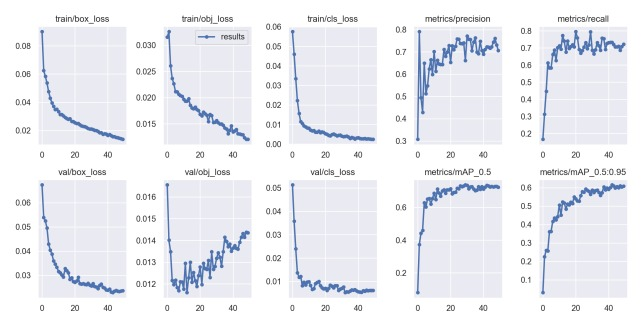
\includegraphics[width=0.7\linewidth]{img/cap3/yolov5artigo.jpeg}
        \caption{YOLOv5 \cite{diascomparaccao}}
        \label{fig:yolov5}
    \end{minipage}
\end{figure}

\begin{figure}[!h]
    \center
    \begin{minipage}{1\linewidth}
        \center
        \captionsetup{justification=centering,margin=0.5cm,font=small}
        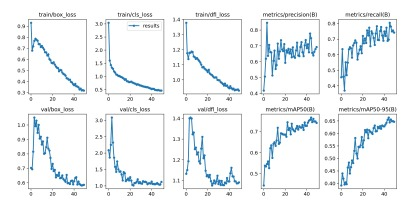
\includegraphics[width=0.7\linewidth]{img/cap3/yolov8artigo.jpeg}
        \caption{YOLOv8 \cite{diascomparaccao}}
        \label{fig:yolov8}
    \end{minipage}
\end{figure}

Este trabalho investigou a importância da detecção de objetos em imagens de áreas rurais, comparando os modelos YOLOv5 e YOLOv8. A detecção precisa de objetos é crucial em várias aplicações agrícolas, de monitoramento e preservação ambiental, aumentando a eficiência, produtividade e sustentabilidade nessas áreas. Os modelos YOLOv5 e YOLOv8 destacaram-se na detecção de objetos em tempo real, com o YOLOv5 sendo eficiente no treinamento e o YOLOv8 se sobressaindo pela precisão na detecção.


\subsection{UAV-YOLOv8: A Small-Object-Detection Model Based on Improved YOLOv8 for UAV Aerial Photography Scenarios}

O artigo de \cite{wang2023uav} se inicia apresentando o crescente uso de VANTs para diversas aplicações da ciência e engenharia. Contudo, devido a altura do voo, o uso de suas imagens para captura de objetos específicos delas mostra-se um desafio, uma vez que a proporção existente entre objeto e a foto como um todo é muito pequena. Além disso, realizar o processamento dessas imagens em tempo real, de maneira embarcada em um VANT, dada as limitações de hardwares desses equipamentos, mostra-se outro desafio. Disto, entende-se que a primeira motivação do trabalho está em melhorar o desempenho da detecção de objetos considerando os recursos limitados da plataforma de hardware.

Para a tarefa de detecção, como nos demais trabalhos citados nessa dissertação, recorre-se às RNC. Entre elas, a principal diferença está na quantidade de estágios de deteção dos algoritmos, que são aqueles que fazem a detecção em dois estágios, como a Fast R-CNN, e também aqueles que a realizam em apenas um, que é o caso da YOLO\cite{girshick2015fast}.

A alteração da arquitetura da RNC influi diretamente no resultado desejado. Contudo, a simples troca de um algoritmo para outro não satisfaz completamente a necessidade de aumentar a acurácia desejada, levando à busca por alterações na estrutura da rede para obter mais interessantes

Assim, o trabalho de \cite{wang2023uav} propõe um modelo de detecção de objetos baseado em fotografias obtidas por meio de VANTs, chamado UAV-YOLOv8, que se vale da  YOLOv8 como rede backbone. No geral, essa nova arquitetura melhora significativamente a precisão e a eficiência da detecção de objetos em imagens capturadas por UAVs, mantendo um baixo consumo de recursos, o que o torna adequado para plataformas de UAVs com capacidades limitadas. Ele é especialmente otimizado para enfrentar os desafios das imagens aéreas, como a detecção de pequenos objetos em fundos complexos.

A oitava versão da YOLO notabiliza-se por ser o estado da arte na ciência de detecção de objetos. Sua estrutura utiliza a arquitetura modificada CSPDarknet53 como backbone, com módulos C2f e SPPF para otimizar a extração e processamento das características de imagem. O neck adota a estrutura PAN-FPN, que melhora a fusão de informações posicionais e semânticas, tornando o modelo mais leve e eficiente. Por fim a head desacoplada usa ramos separados para classificação e regressão de caixas, melhorando a precisão e a robustez da detecção, sem o uso de âncoras \cite{redmon2018yolov3}.

Neste artigo, então, para melhorar sua eficácia nesses cenários, o foi proposta uma otimização do modelo utilizando a função de perda WIoU v3, que aprimora a generalização; o mecanismo de atenção BiFormer, que foca em características de alta relevância; e o módulo de processamento de características FFNB, que melhora a fusão de características de diferentes escalas. Essas melhorias resultaram no UAV-YOLOv8, que expande a detecção de 3 para 5 escalas, aprimorando significativamente a detecção de pequenos objetos.

A experimentação do novo modelo foi proposta de forma a avaliar a precisão de detecção de objetos pequenos e a eficiência de recursos do modelo proposto, UAV-YOLOv8s. Como dataset, o estudo fez uso do dataset VisDrone2019, que inclui fotografias aéreas obtidas por UAVs em várias cidades da China, capturando diferentes cenários e condições de iluminação. Escolheu-se o VisDrone2019 devido à sua riqueza de informações e diversidade. Foi desenvolvido pela Universidade de Tianjin e inclui uma variedade de categorias de objetos de detecção e distribuições variadas de objetos, abrangendo tanto cenários com alta quanto baixa densidade de objetos, e fotos tiradas durante o dia e a noite.

Assim, para a detecção de objetos em fotos capturadas por VANTs, em se tratando de objetos muitos, fundos complexos e recursos de hardware limitados, há um desafio em manter a alta a precisão dos modelos. O UAV-YOLOv8, baseado no YOLOv8, é proposto para otimizar a detecção, introduzindo a função de perda WIoU v3 e o mecanismo de atenção BiFormer, melhorando o foco do modelo e reduzindo a perda de detecção de objetos pequenos. O modelo aprimorado alcança um aumento médio de 7,7\% (Figura\ref{fig:chines}) na precisão sem aumentar seu tamanho, mas a adição de duas camadas de detecção aumenta a complexidade e o tempo de computação. Comparado com outros modelos mainstream, o UAV-YOLOv8 demonstrou desempenho superior, de modo geral (Figura \ref{fig:chines-tabela}). A precisão ainda é baixa para objetos muito pequenos, como bicicletas, e futuras pesquisas seriam necessárias na otimização dessa precisão, podendo elas ficarem na confecção do dataset para melhores resultados, alteração da arquitetura, entre outras abordagens.

\begin{figure}[!h]
    \center
    \begin{minipage}{1\linewidth}
        \center
        \captionsetup{justification=centering,margin=0.5cm,font=small}
        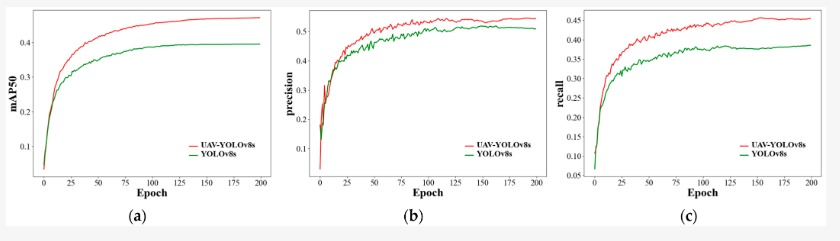
\includegraphics[width=0.7\linewidth]{img/cap3/chines.jpeg}
        \caption{Comparação da YOLOv8 com a rede modificada}
        \label{fig:chines}
    \end{minipage}
\end{figure}

\begin{figure}[!h]
    \center
    \begin{minipage}{1\linewidth}
        \center
        \captionsetup{justification=centering,margin=0.5cm,font=small}
        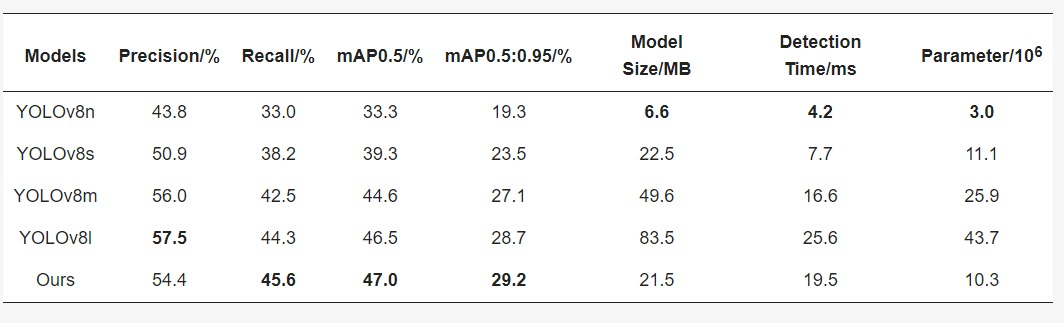
\includegraphics[width=0.7\linewidth]{img/cap3/chines-tabela.jpeg}
        \caption{Comparação da YOLOv8 com a rede modificada}
        \label{fig:chines-tabela}
    \end{minipage}
\end{figure}

\section{Considerações Finais}

A Tabela \ref{tab:relacionado1} apresenta um resumo de todos os trabalhos relacionados descritos neste capítulo, considerando os seguintes temas:

\begin{itemize}
    \item \textit{Treinamento utilizando YOLOv8}: Utilização de RNC para realizar treinamento em conjuntos de imagens;
    \item \textit{Alteração de Parâmetros da RNC para treinamento}: Variação de parâmetros como batch size e otimizadores para treinamento;
    \item \textit{Utilização de VANT}: Coleta de fotos utilizando VANTs;
    \item \textit{Subestações de Energia}: Coleta, treinamento e inserção voltada para subestações de energia;
    \item \textit{Automação de Inserção de RV}: Construção de sistema de inserção automática de objetos em um sistema de RV.
\end{itemize}

\begin{table}[!hbt]
    \centering
    \caption{Resumo comparativo dos trabalhos relacionados}
    \begin{tabular}{ >{\centering\arraybackslash}m{5cm} | >{\centering\arraybackslash}m{2cm} | >{\centering\arraybackslash}m{2cm} | >{\centering\arraybackslash}m{2cm} | >{\centering\arraybackslash}m{2cm} | >{\centering\arraybackslash}m{2cm} }
    \hline
    \cellcolor[gray]{0.9} \textbf{Trabalhos Relacionados} & 
    \cellcolor[gray]{0.9} \begin{sideways} \textbf{Alteração de Parâmetros da RNC} \end{sideways} & 
    \cellcolor[gray]{0.9} \begin{sideways} \textbf{Treinamento utilizando YOLOv8} \end{sideways} & 
    \cellcolor[gray]{0.9} \begin{sideways} \textbf{Utilização de VANT} \end{sideways} & 
    \cellcolor[gray]{0.9} \begin{sideways} \textbf{Subestações de Energia} \end{sideways} &
    \cellcolor[gray]{0.9} \begin{sideways} \textbf{Automação de Inserção de RV} \end{sideways} \\
    \hline 
    \cite{gonzaga2023identificaccao} & \textcolor{green}{\(\checkmark\)} & \textcolor{green}{\(\checkmark\)} & \textcolor{red}{\(\times\)} & \textcolor{red}{\(\times\)} & \textcolor{red}{\(\times\)} \\
    \hline
    \cite{diascomparaccao} & \textcolor{green}{\(\checkmark\)} & \textcolor{green}{\(\checkmark\)} & \textcolor{red}{\(\times\)} & \textcolor{red}{\(\times\)} & \textcolor{red}{\(\times\)} \\
    \hline
    \cite{wang2023uav} & \textcolor{green}{\(\checkmark\)} & \textcolor{green}{\(\checkmark\)} & \textcolor{green}{\(\checkmark\)} & \textcolor{red}{\(\times\)} & \textcolor{red}{\(\times\)} \\
    \hline
    (ZUZA, 2024) & \textcolor{green}{\(\checkmark\)} & \textcolor{green}{\(\checkmark\)} & \textcolor{green}{\(\checkmark\)} & \textcolor{green}{\(\checkmark\)} & \textcolor{green}{\(\checkmark\)} \\
    \end{tabular}
    \label{tab:relacionado1}
\end{table}

Pela análise da Tabela \ref{tab:relacionado1}, entende-se que não há ainda um trabalho que reúna todos os tópicos apresentados. É fato que há diversos trabalhos que exploram a detecção de objetos em diversos cenários, utilizando diversas versões da YOLO, inclusive utilizando VANT, para obtenção de imagens. Contudo, no contexto de subestações de energia e identificação de seus equipamentos, há uma lacuna de contribuições. Naturalmente, isso mostra o quão prolífico esta dissertação se mostra, ao unir todas essas áreas de estudo num propósito ainda não explorado.

No próximo capítulo, serão detalhados os materiais e métodos utilizados para a solução proposta.














